\documentclass[12pt]{article}
\usepackage{minted}
\usepackage[pdftex]{graphicx}
\usemintedstyle{emacs}

%opening
\title{Grammatical Framework Assignment\\Chatbot implementation with variants}
\author{Thuong-Hai Pham}
\date{July 11, 2017}

\begin{document}

\maketitle

\section{Introduction} \label{introduction}

In the recent years, conversational agents (chatbots) are increasing their importance by approaching many aspects of the technology industry, especially E-commerce. When it comes to implementing a chatbot that will be used in real life, the developers usually construct a work flow of which question the chatbot has to ask the user to acquire adequate information that can lead to a decision or action.

However, taking the advantage of a feature in Grammatical Framework (GF) \cite{ranta2004grammatical} - the variants parameter, we can instruct the chatbot to construct its work flow without explicit step-by-step declaration. Consequently, we implemented a web-based chatbot for customers to order Subway\textsuperscript{\textregistered} as a demonstration. 


\section{Grammar}
As mentioned in Section \ref{introduction}, it is a common practice to manually construct a work flow for chatbots to acquire information from user through natural language interaction.

For example:
\begin{enumerate}
    \item Greeting
    \item Which kind of item the user would like to have?
    \item How many items of that kind are ordered?
    \item What additional components should go with those items?
    \item Do the user would like to order other kinds? If yes, go back to step 2.
    \item Confirmation.
\end{enumerate}

In contrast, by making use of GF variant, \cite{bringert2007rapid} delegated the work flow construction to GF itself. The variants parameter in GF allow the sentence to be partially input.

\begin{listing}[ht]
	\begin{minted}[frame=single]{haskell}
drink n s t = { s = giveMe ++
		variants { n.s ++ s.s ++ t.s!n.n; 
				  n.s ++ t.s!n.n } 
		++ please } ;
	\end{minted}
	\caption{Drink order with variants}
\end{listing}

As in the code snippet above, the drink order is defined with variants parameter, accepts two different input forms, with or without s.s (drink size). Hence, the user can order "one coke" or "one small coke". This missing size, when being parsed, gives us a metavariable (denoted by ?).

\begin{minted}[frame=single]{haskell}
Subway> parse "a coke"
order drink (drinkNumber num_1) ?3 coke
Subway> parse "a coke" | linearize
one ?3 coke
\end{minted}

We will deal with this metavariable in the next section.

\section{Implementation}
After accepting input with variants as in the previous section, GF parser gives us a parse of the order with many metavariables needed to be filled. This mechanism helps us to automatically generate questions to be asked without following a manual work flow. To "fill" the order, our Python code:

\begin{enumerate}
    \item Traverses throughout the parse structure with unpack function.
    \item Identifies each metavariable
    \item Generates the corresponding question to be asked.
    \item Waits for response from user, then fill the variable with that response if valid.
\end{enumerate}


Although we do not explicitly define each step the chatbot need to interact with the user, the steps above to automatically generate work flow also requires some predefined states to control the generation of work flow while keeping the interaction with user: STATE\_IDLE, STATE\_FILLING, STATE\_RECEIVING, STATE\_DONE. These states allows the chatbot to play a role-based game with user and knows what it is going to do next simultaneously.

In addition, when generating questions, the chatbot also refers to that item (Figure \ref{fig:demo}) to prevent user from being confused when ordering multiple items.

This chatbot also inherits a very strong advantage of GF to develop a multilingual capability. For demonstration, we implemented the English and Vietnamese version of the chatbot by defining two concrete grammar SubwayEng.gf and SubwayVie.gf. The expansion to other languages would take little effort to complete.

\section{Demonstration}

\subsection{Installation} 
The installation process is described step-by-step in README.md in the source code. In general, this chatbot only requires Python, GF library, GF Python API and Flask (a Python package to build light-weight website).


\subsection{Example} 
Figure \ref{fig:demo} shows a sample dialogue between a user and our Subway chatbot. The chatbot was trying to fill in the blank from previous information. At the same time, in each question, it re-mentioned the item to prevent ambiguity when the user ordered multiple items in one sentence.
\begin{figure}[ht]
    \caption{Example of a dialogue with Subway Chatbot}
    \centering
	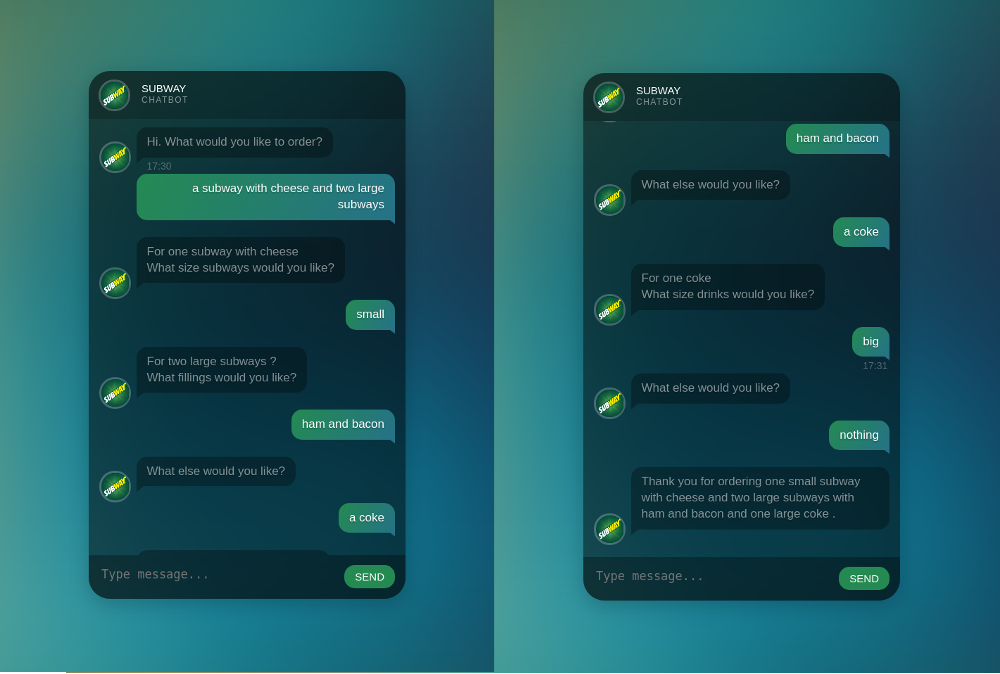
\includegraphics[width=\textwidth]{exported}
	\label{fig:demo}
\end{figure}

\section{Conclusion}
In conclusion, GF variants parameter is a very efficient and neat feature when we apply GF in implementing a chatbot by eliminating manual constructed work flow of the chatbot. Moreover, this application is also inherited from GF the multilingual capability, hence, reduces the amount of work to expand the application to other languages.

However, there is one drawback of the GF API, in which it is not well documented. For example, in the case of Python (which is a very popular language), the document is short and somehow outdated by showing that parse with cat parameter is a string, while it should be pgf.Type. This lead to a lot of effort being put on not to construct the grammar but to read the source code and try-and-error with the API.

Yet in general, applying GF helps to reduce significant amount of work, allows one individual to implement a commercial chatbot without any chatbot framework and supports effortless multilingual extension.


\bibliographystyle{apalike}
\bibliography{gf-report}

\end{document}
